\section{Temporal Graph Reasoning Benchmark: 
\benchmarkname}\label{sec:tgrab}

 % {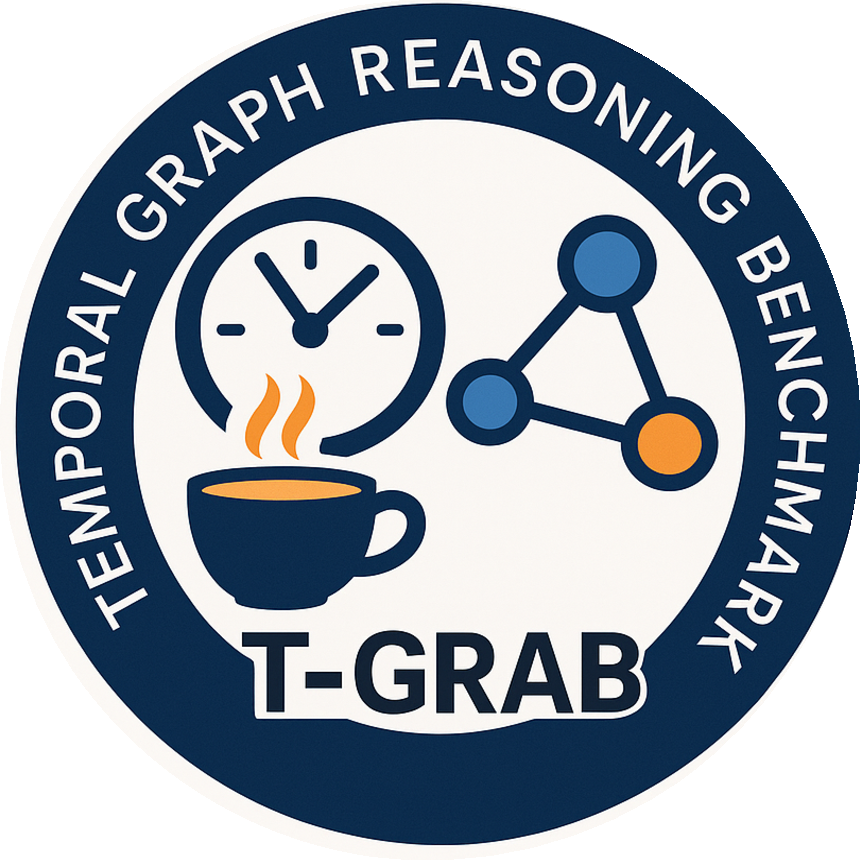
\includegraphics[height=1.5mm]{kdd/figs/logo.pdf}
 % }

\looseness-1 In this section, we introduce the Temporal Graph Reasoning Benchmark~(T-GRAB), the first synthetic benchmark designed to systematically evaluate the temporal reasoning capabilities of TGNNs in a controlled environment. \benchmarkname comprises three categories of dynamic link prediction tasks, each probing distinct aspects of temporal reasoning: 1) \emph{periodicity} tasks, which assess counting and memorization capabilities; 2) \emph{cause-and-effect} tasks, which evaluate the ability to identify causal relationships across time delays; and 3) \emph{long-range dependencies} tasks, which measure how effectively models capture dependencies spanning both spatial and temporal dimensions~\changed{(here \emph{spatial} refers to the graph structure}). These task families are examined in detail in Sections~\ref{synth-benchmark:periodicity}, ~\ref{synth-benchmark:cause}, and ~\ref{synth-benchmark:long}, respectively. As summarized in \Cref{tab:data}, \benchmarkname encompasses a diverse spectrum of graph characteristics and temporal patterns, providing a comprehensive framework to rigorously test the fundamental reasoning capabilities of TGNNs.

\begin{table}[t]
\caption{\benchmarkname tasks characteristics. } \label{tab:data} 
  \resizebox{\linewidth}{!}{%
  \begin{tabular}{ l | ccc}
  \toprule
  Task & Counting & Memorizing & \begin{tabular}{cc}
       Spatial  \\ Understanding
  \end{tabular}  \\ 
  \midrule
  Periodicity & \cmark & \cmark & \xmark\\ 
  Cause-and-Effect & \xmark & \cmark & \xmark\\ 
  Long-Range Dependencies & \xmark & \cmark & \cmark\\ 
  \bottomrule
  \end{tabular}
  }
\end{table}

\begin{figure*}[!t]
    \centering
    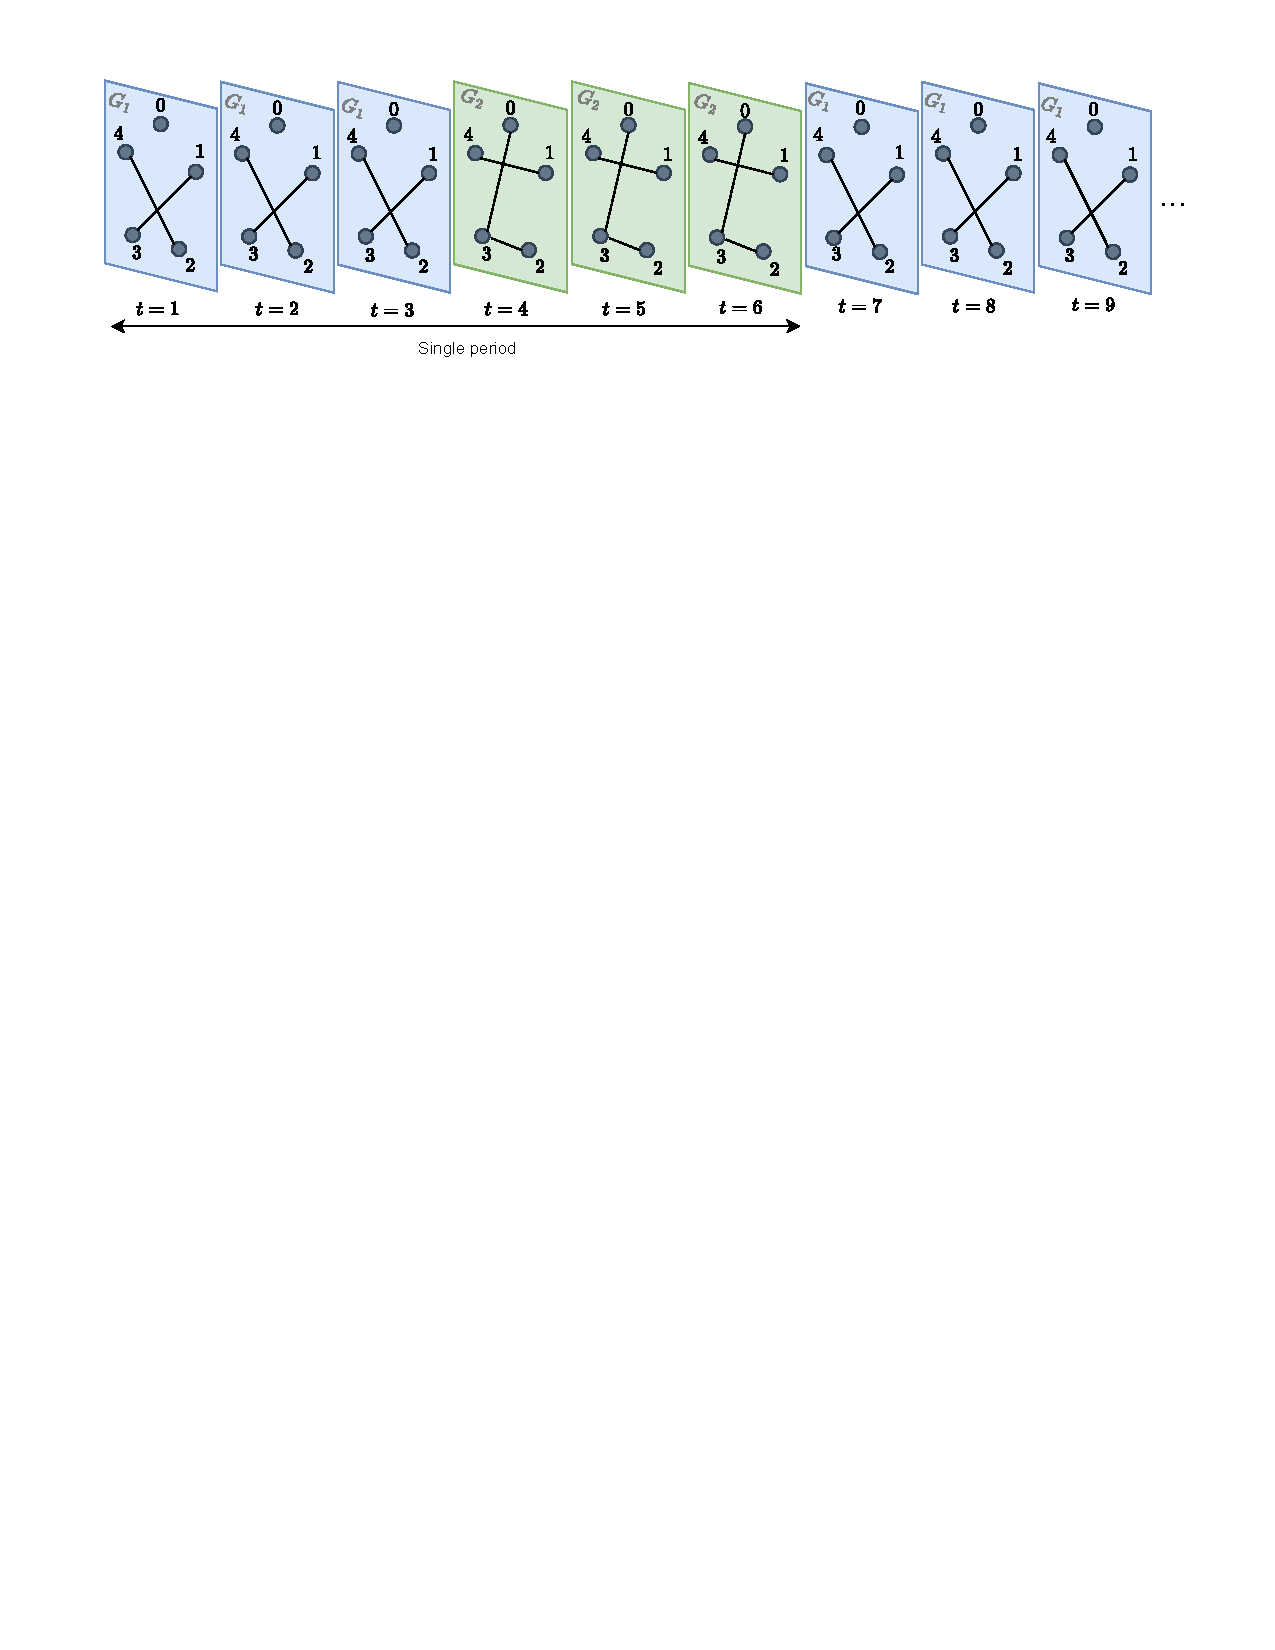
\includegraphics[width=0.75\linewidth,  keepaspectratio]{figs/periodicity/Fixed_ER/(2, 3)_dataset.pdf}
    \caption{Periodic task in $\Pdet{k\!=\!2,n\!=\!3}$ with 2 unique snapshots repeated 3 times within a period. }
    \label{fig:periodicity}
\end{figure*}

% Table~\ref{tab:data} provides an overview of the statistics and characteristics of the datasets introduced in \benchmarkname. Table~\ref{tab:data} shows that \benchmarkname covers a diverse range of dataset statistics and associated tasks to test the limit of TGNNs.

\looseness-1 \textbf{Methods in Comparison.} We conduct a comprehensive evaluation of diverse Temporal Graph Learning (TGL) approaches on \benchmarkname tasks. Our analysis encompasses four continuous-time (CTDG) architectures (DyGFormer~\cite{dygformer}, CTAN~\cite{ctan}, TGN~\cite{tgn}, and TGAT~\cite{tgat}), three discrete-time (DTDG) frameworks (EvolveGCN \cite{evolvegcn}, T-GCN~\cite{tgcn}, and GC-LSTM~\cite{gclstm}), two static graph methods (GCN~\citep{gcn} and GAT~\citep{gat}), for which we use their DTDG implementations provided by UTG~\citep{huangutg}, and two established baselines (the \textit{persistence} heuristic, which predicts edges from the previous timestep, and $\text{Edgebank}_{\infty}$~\citep{poursafaei2022betterevaluationdynamiclink}, a pure memorization heuristic that predicts True if it has seen that edge in the past and False otherwise.). This selection represents the state-of-the-art across different temporal graph learning paradigms, enabling a rigorous assessment of their fundamental reasoning capabilities. 

% \ah{we need to add some details of how we apply CTDG methods on DTDG datasets. We can discuss here if we have space or put it in experiment details.}
% \gr{There is one or two small sentences at the end of Sec 3 about this, we can add more details in appendix indeed.  }



\textbf{Evaluation Protocols.}
Prior research has demonstrated that evaluation results for dynamic link prediction can vary substantially depending on negative sampling strategies~\cite{poursafaei2022betterevaluationdynamiclink}. To ensure methodological rigor and reproducibility, we implement a comprehensive evaluation framework that calculates the average $F_1$ score across all possible node pairs at each test time step. This approach eliminates sampling bias and provides a more reliable performance assessment. For periodicity tasks, our evaluation incorporates all test edges in the $F_1$ calculation to capture the full spectrum of temporal patterns. In contrast, for cause-and-effect and long-range dependencies tasks, we restrict the evaluation to edges involving the memory/target node, as they are the only predictable connections within the otherwise stochastically generated graph. This targeted evaluation ensures that model performance reflects genuine temporal reasoning capabilities rather than chance correlations in random edge formations.


% Since the dynamic graphs we consider are relatively small, we do not have to rely on negative sampling for our evaluation, which has many drawbacks~\cite{poursafaei2022betterevaluationdynamiclink}, and instead evaluate the models by reporting the average $F_1$ score over all possible edges across all time steps in the test set.  For the periodicity tasks, all edges in the test set are included in the $F_1$ computation. For the  cause and effect and long range tasks, not all edges are included in the $F_1$ computation since only the edges involving the memory node can be predicted. Indeed, all the other edges are generated completely at random. Hence, for these tasks the $F_1$ is averaged only over the edges of the test set involving the memory node. 